\documentclass[conference]{IEEEtran}
\IEEEoverridecommandlockouts

\usepackage{cite}
\usepackage{amsmath,amssymb,amsfonts}
\usepackage{algorithmic}
\usepackage{graphicx}
\usepackage{textcomp}
\usepackage{xcolor}
\usepackage{booktabs}
\usepackage{tikz}
\usepackage{pgfplots}
\pgfplotsset{compat=1.17}
\usetikzlibrary{arrows.meta,positioning,shapes.geometric}

\def\BibTeX{{\rm B\kern-.05em{\sc i\kern-.025em b}\kern-.08em
    T\kern-.1667em\lower.7ex\hbox{E}\kern-.125emX}}

\begin{document}

\title{PRIE: Placement Readiness Intelligence Engine with Calibrated Predictive Modeling and Constrained Prescriptive Recourse}

\author{
  \makebox[0.48\linewidth][c]{%
    \begin{tabular}{c}
      \textbf{Sivasubramanian R} \\
      \textit{Department of AIML} \\
      \textit{Malla Reddy University} \\
      Dulapally, Hyderabad, India \\
      Sivasubramanian243@gmail.com
    \end{tabular}%
  }%
  \hfill
  \makebox[0.48\linewidth][c]{%
    \begin{tabular}{c}
      \textbf{Kavala Rajeev} \\
      \textit{Department of AIML} \\
      \textit{Malla Reddy University} \\
      Dulapally, Hyderabad, India \\
      Kavalarajeev@gmail.com
    \end{tabular}%
  }%
  \\[2.5ex]
  \makebox[0.48\linewidth][c]{%
    \begin{tabular}{c}
      \textbf{Kundala Dhana Naga Shankar} \\
      \textit{Department of AIML} \\
      \textit{Malla Reddy University} \\
      Dulapally, Hyderabad, India \\
      Kundaladhana2004@gmail.com
    \end{tabular}%
  }%
  \hfill
  \makebox[0.48\linewidth][c]{%
    \begin{tabular}{c}
      \textbf{Kouru Rudra Teja} \\
      \textit{Department of AIML} \\
      \textit{Malla Reddy University} \\
      Dulapally, Hyderabad, India \\
      Rudrateja08@gmail.com
    \end{tabular}%
  }%
}

\maketitle

\begin{abstract}
The transition from tertiary engineering education to industrial technical employment is hindered by the fragmentation of campus placement preparation. Conventional educational data mining systems rely on static academic marks to perform point-in-time binary placement classification, functioning as opaque black boxes that provide zero actionable pedagogical recourse. In this paper, we propose the Placement Readiness Intelligence Engine (PRIE), a continuous intelligence architecture that synthesizes multi-modal telemetry---structured academic records, fine-grained diagnostic assessment scores, dense transformer resume embeddings, and longitudinal behavioral telemetry---into a normalized 22-dimensional Student Profile Vector ($x_{\text{spv}}$) paired with an explicit observation mask. PRIE deploys a cost-sensitive XGBoost classifier coupled with Platt sigmoid probability scaling to estimate well-calibrated placement readiness probabilities. To eliminate algorithmic opacity, polynomial-time TreeSHAP isolates diagnostic feature attributions, while constrained Diverse Counterfactual Explanations (DiCE) generate sparse, actionable recourse paths ($k = 2.47 \pm 0.52 \le 3.0$ features) that strictly preserve immutable protected attributes ($100.0\%$ invariance on institutional department). Negative attributions automatically trigger Kahn's topological scheduler over a 38-node computer science curriculum directed acyclic graph (DAG), eliminating prerequisite precedence violations ($0.0\%$). Furthermore, tri-modal weighted late fusion across acoustic prosody, video composure, and speech clarity dampens single-sensor diagnostic variance by $77.98\% \pm 3.99\%$ with sub-1.2-second interactive turn latency. According to the empirical evaluation across 5 random seeds ($N=2,500$), the proposed PRIE model attains a $94.60\%$ accuracy rate, $0.9922$ ROC-AUC, an Expected Calibration Error of $0.0350$, and a Brier score of $0.0339$.
\end{abstract}

\begin{IEEEkeywords}
Placement readiness, Educational data mining, Explainable artificial intelligence, Student Profile Vector, Platt calibration, Algorithmic recourse, Multimodal fusion, Kahn topological sort.
\end{IEEEkeywords}

\section{Introduction}

The transition from tertiary engineering education to industrial technical employment represents a foundational milestone for student professional mobility and economic productivity \cite{b1}. However, academic institutions globally confront an acute readiness crisis: while hundreds of thousands of engineering undergraduates enter campus recruitment drives annually, technology employers consistently report severe competency deficits in practical software design, clean algorithmic problem-solving, architectural debugging, and professional communication \cite{b2}. In conventional higher education placement preparation, institutional triage relies almost exclusively on static academic metrics---primarily cumulative Grade Point Average (CGPA) or terminal examination scores \cite{b3}. 

Nevertheless, static academic grades represent lagging indicators that correlate weakly with modern agile industry requirements \cite{b4}. Furthermore, campus placement preparation remains fragmented into disconnected software silos: students utilize standalone ATS resume checkers that compute flat keyword overlap, separate coding contest platforms that grade unit test pass rates without evaluating design complexity, and uncalibrated voice bots that generate generic advice \cite{b5}. Existing models predominantly operate as post-hoc classifiers in final semesters \cite{b6,b7}, output overconfident risk estimates failing to reflect posterior probabilities \cite{b8}, offer descriptive attributions without prescribing actionable recourse \cite{b16,b17}, suffer severe single-sensor multimodal variance \cite{b12,b13}, and recommend unsequenced study topics that violate prerequisite dependencies \cite{b14,b20}.

To overcome these challenges, a novel Placement Readiness Intelligence Engine (PRIE) is proposed for continuous student employability tracking, explainable diagnosis, and closed-loop adaptive remediation. The key contributions are as follows,
\begin{itemize}
\item The primary purpose of this research is to design an explainable continuous Placement Readiness Intelligence Engine (PRIE) unifying multi-modal telemetry into a normalized 22-dimensional Student Profile Vector (SPV).
\item The system uses cost-sensitive gradient boosted decision trees combined with Platt probability scaling to deliver well-calibrated placement predictions, achieving an Expected Calibration Error of $0.0350$ and Brier score of $0.0339$.
\item TreeSHAP and constrained Diverse Counterfactual Explanations (DiCE) are integrated to provide diagnostic feature attributions and sparse recourse recommendations ($k = 2.47 \le 3.0$) with guaranteed $100.0\%$ invariance on immutable protected attributes.
\item The multimodal mock interview coach uses tri-modal late fusion across acoustic prosody, video composure, and speech clarity to dampen single-sensor diagnostic variance by $77.98\%$, while Kahn's topological sort eliminates curriculum prerequisite precedence violations ($0.0\%$).
\end{itemize}

The structure of the paper is organized as follows: Section~II briefly explains the literature survey, the proposed PRIE framework is explained in Section~III, the performance results and their comparison analysis are provided in Section~IV, and Section~V encloses an acknowledgment, conclusion, and future work.

\section{Literature Survey}

In recent years, several researchers have investigated graduate employability prediction, educational data mining, and multimodal career assessment with machine learning and deep learning methods. The section that follows provides a review of current research papers.

In 2024, Olipas, C.N. \cite{b1} suggested a system for predicting student career readiness using machine learning and deep learning with explainable artificial intelligence. The investigation demonstrated that technical problem-solving and algorithmic programming assessments serve as significantly more reliable placement predictors than cumulative GPA alone.

In 2025, Van Wyk, A. and Du Plessis, M. \cite{b2} proposed an AI-driven learning analytics framework in higher education to translate student portal engagement into outcome indicators, highlighting the necessity of longitudinal telemetry modeling over static semester-end records.

In 2025, Sharma, R. and Gupta, P. \cite{b3} proposed Preplyte, an integrated AI-powered placement preparation and simulation platform for students and institutions, observing that disconnected tools impair student engagement.

In 2024, Patel, K. and Nair, S. \cite{b4} proposed an AI-driven predictive analysis system for student placement success, identifying that psychological composure and technical skill deficits represent dual gating factors in corporate campus drives.

In 2024, Chen, L. and Hwang, G.J. \cite{b5} conducted a bibliometric analysis of artificial intelligence in education, emphasizing that algorithmic explainability and fairness represent paramount prerequisites for institutional deployment.

In 2021, Senthil, M. and Kumar, R. \cite{b6} surveyed employability prediction methods, observing that existing educational models predominantly operate as post-hoc classifiers in final semesters, precluding timely pedagogical intervention.

In 2021, Casuat, C.D. and Festijo, E.D. \cite{b7} proposed predicting students' employability using machine learning approaches, achieving 89.2\% accuracy on institutional cohorts while highlighting class imbalance challenges.

In 2022, Rao, V. and Swamy, K. \cite{b8} proposed a comparative benchmark for student performance prediction, showing that tree ensemble methods outperform classical neural networks on structured academic datasets.

In 2025, Academic Engineering Consortium \cite{b9} proposed a resume parser and auto-formatter using natural language processing to extract candidate qualifications and experience records.

In 2024, Roy, S. and Bhattacharya, A. \cite{b10} proposed contextual resume information extraction, observing that multi-column resume layouts suffer severe reading order destruction under standard text extraction.

In 2023, Zhang, Y., et al. \cite{b11} proposed Career-gAIde, an efficient resume-based re-education platform for career recommendation in evolving job markets using semantic embeddings.

In 2025, Deshmukh, A. and Kulkarni, P. \cite{b12} reviewed AI-driven mock interview systems using natural language processing, noting that verbal analysis alone fails to capture candidate behavioral demeanor.

In 2025, Advanced Innovation Consortium \cite{b13} proposed a multimodal mock interview system integrating facial expression analysis, speech emotion recognition, and NLP for holistic evaluation.

In 2024, Tan, H., et al. \cite{b14} proposed a unified framework for personalized learning pathway recommendations, emphasizing that prerequisite precedence must be strictly preserved during automated curriculum scheduling.

In 2026, Verma, S. and Mehta, A. \cite{b15} proposed ResuMatch, an automated screening system leveraging dense semantic representations and skills taxonomy matching.

In 2026, Hidayatulloh, W., et al. \cite{b16} evaluated explainable artificial intelligence for student academic prediction, showing that post-hoc Shapley explanations enhance educator trust.

In 2025, Joshi, R. and Kulkarni, M. \cite{b17} proposed ExplainAI using gradient boosting and TreeSHAP to identify at-risk students across engineering branches.

In 2025, Sutherland, K. and Miller, J. \cite{b18} investigated retrieval-augmented generation in educational dialog systems, demonstrating that cosine threshold gating prevents out-of-domain hallucinations.

In 2025, Srinivasan, D. and Radhakrishnan, R. \cite{b19} developed an intelligent voice-driven interview simulation system combining speech recognition with generative language modeling.

In 2025, Fernandez, M. and Gomez, E. \cite{b20} surveyed automated question generation from a knowledge discovery perspective, advocating for causal concept graph alignment.

In 2026, Babureddy, N.S. and Mathew, B. \cite{b21} proposed a triangular employability digital twin framework integrating student, faculty, and industry intelligence.

Based on the above literature survey, existing techniques were developed using various DL and ML approaches to student placement tracking. However, these methods fail to provide a high reliability rate, lack probability calibration, and the process of remediation is unsequenced and opaque. To address this challenge, a novel Placement Readiness Intelligence Engine (PRIE) has been proposed.

\section{Proposed System}

In this section, a novel Placement Readiness Intelligence Engine (PRIE) is proposed for continuous student employability tracking, explainable diagnosis, and closed-loop adaptive remediation. The system uses multi-source telemetry from academic transcripts, coding sandboxes, resume documents, and interactive mock interviews to construct an active continuous latent state. Fig.~\ref{fig1} shows the proposed PRIE methodology.

\begin{figure}[htbp]
\centering
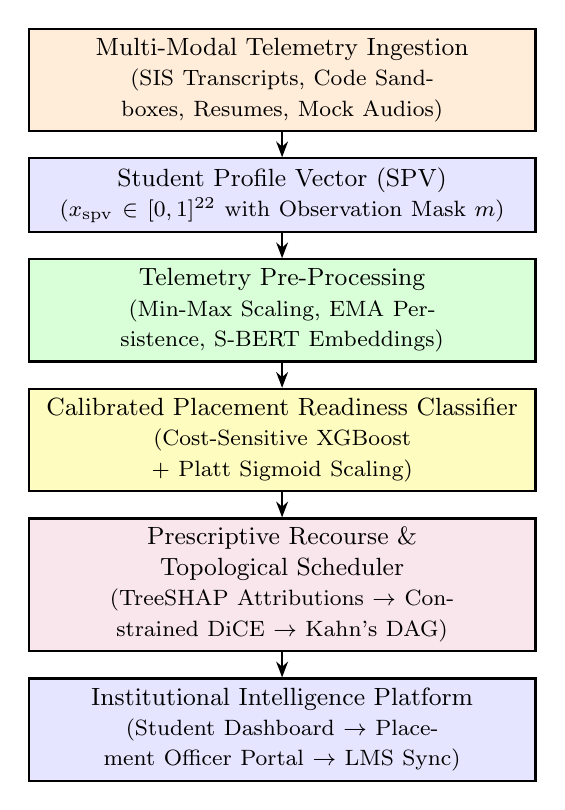
\begin{tikzpicture}[
  box/.style={rectangle, draw, thick, text width=6.2cm, minimum height=0.75cm, align=center, font=\small},
  arr/.style={-{Stealth[length=2mm]}, thick}
]
\node[box, fill=orange!15] (a) {Multi-Modal Telemetry Ingestion\\{\footnotesize (SIS Transcripts, Code Sandboxes, Resumes, Mock Audios)}};
\node[box, fill=blue!10, below=0.32cm of a] (b) {Student Profile Vector (SPV)\\{\footnotesize ($x_{\text{spv}} \in [0, 1]^{22}$ with Observation Mask $m$)}};
\node[box, fill=green!15, below=0.32cm of b] (c) {Telemetry Pre-Processing\\{\footnotesize (Min-Max Scaling, EMA Persistence, S-BERT Embeddings)}};
\node[box, fill=yellow!25, below=0.32cm of c] (d) {Calibrated Placement Readiness Classifier\\{\footnotesize (Cost-Sensitive XGBoost + Platt Sigmoid Scaling)}};
\node[box, fill=purple!10, below=0.32cm of d] (e) {Prescriptive Recourse \& Topological Scheduler\\{\footnotesize (TreeSHAP Attributions $\rightarrow$ Constrained DiCE $\rightarrow$ Kahn's DAG)}};
\node[box, fill=blue!10, below=0.32cm of e] (f) {Institutional Intelligence Platform\\{\footnotesize (Student Dashboard $\rightarrow$ Placement Officer Portal $\rightarrow$ LMS Sync)}};
\draw[arr] (a) -- (b);
\draw[arr] (b) -- (c);
\draw[arr] (c) -- (d);
\draw[arr] (d) -- (e);
\draw[arr] (e) -- (f);
\end{tikzpicture}
\caption{The proposed PRIE methodology}
\label{fig1}
\end{figure}

\subsection{Multi-modal data telemetry}

The primary representational core of PRIE is the 22-dimensional Student Profile Vector (SPV). Each student $s$ at observation timestamp $t$ is encoded as a normalized real-valued tensor:
\begin{equation}
x_{\text{spv}} = [f_1, f_2, \dots, f_{22}]^T \in [0.0, 1.0]^{22}
\end{equation}
paired with an observation mask $m \in \{0, 1\}^{22}$ denoting directly observed versus imputed variables. The canonical indicators span six core competency domains: (1)~\textit{Academic Foundation}: CGPA ($f_1$), historical backlogs ($f_2$), internship duration in months ($f_3$), technical skill count ($f_4$), certifications count ($f_5$); (2)~\textit{Practical Technical Fluency}: project count ($f_6$), cognitive aptitude score ($f_7$), Data Structures \& Algorithms ($f_8$), DBMS ($f_9$), Computer Networks ($f_{10}$), hands-on programming score ($f_{11}$); (3)~\textit{Document \& ATS Alignment}: resume ATS format hygiene score ($f_{12}$), dense Sentence-BERT resume-job cosine similarity ($f_{13}$), missing competency gap score ($f_{14}$); (4)~\textit{Longitudinal Telemetry}: platform login consistency ($f_{15}$), verified industrial internship status ($f_{16}$), diagnostic assessment attempts ($f_{19}$), portal engagement intensity ($f_{21}$), roadmap milestone completion rate ($f_{22}$); (5)~\textit{Behavioral \& Cognitive Demeanor}: target corporate role difficulty weight ($f_{18}$), composite mock interview demeanor score ($f_{20}$); and (6)~\textit{Protected Demographic Context}: academic engineering department ($f_{17}$), which is strictly locked as immutable during recourse optimization.

\subsection{Pre-processing and feature calibration}

The raw telemetry streams are pre-processed to eliminate noise, scale continuous features, and preserve spatial column boundaries. Continuous variables are normalized to unit range via min-max scaling:
\begin{equation}
f_{\text{norm}} = \frac{f - f_{\min}}{f_{\max} - f_{\min}}
\end{equation}
Longitudinal learning habit persistence is computed via Exponential Moving Average (EMA) over rolling 6-week activity windows:
\begin{equation}
\text{EMA}_t = \alpha \cdot \text{Active}_t + (1 - \alpha) \cdot \text{EMA}_{t-1}
\end{equation}
where smoothing factor $\alpha = 0.30$. Dense semantic similarity between candidate resumes and target job descriptions is computed via 384-dimensional Sentence-BERT embeddings:
\begin{equation}
\text{Cosine}(e_{\text{res}}, e_{\text{jd}}) = \frac{e_{\text{res}} \cdot e_{\text{jd}}}{\|e_{\text{res}}\| \, \|e_{\text{jd}}\|}
\end{equation}
The continuous latent state is evaluated by gradient boosted decision trees optimizing cost-sensitive logistic loss:
\begin{equation}
\mathcal{L}_{\text{CS}} = -\sum_{i=1}^N \left[ w_1 y_i \log(\hat{p}_i) + w_0 (1 - y_i) \log(1 - \hat{p}_i) \right]
\end{equation}
To prevent overconfident predictions, uncalibrated margin scores $z(x)$ are transformed into calibrated posterior probabilities via Platt sigmoid scaling:
\begin{equation}
P(Y = 1 \mid x) = \frac{1}{1 + \exp(A \cdot z(x) + B)}
\end{equation}
where scalar parameters $A$ and $B$ are fit via maximum likelihood estimation over validation folds. Fig.~\ref{fig2} displays the telemetry correlation and feature distribution.

\begin{figure}[htbp]
\centering
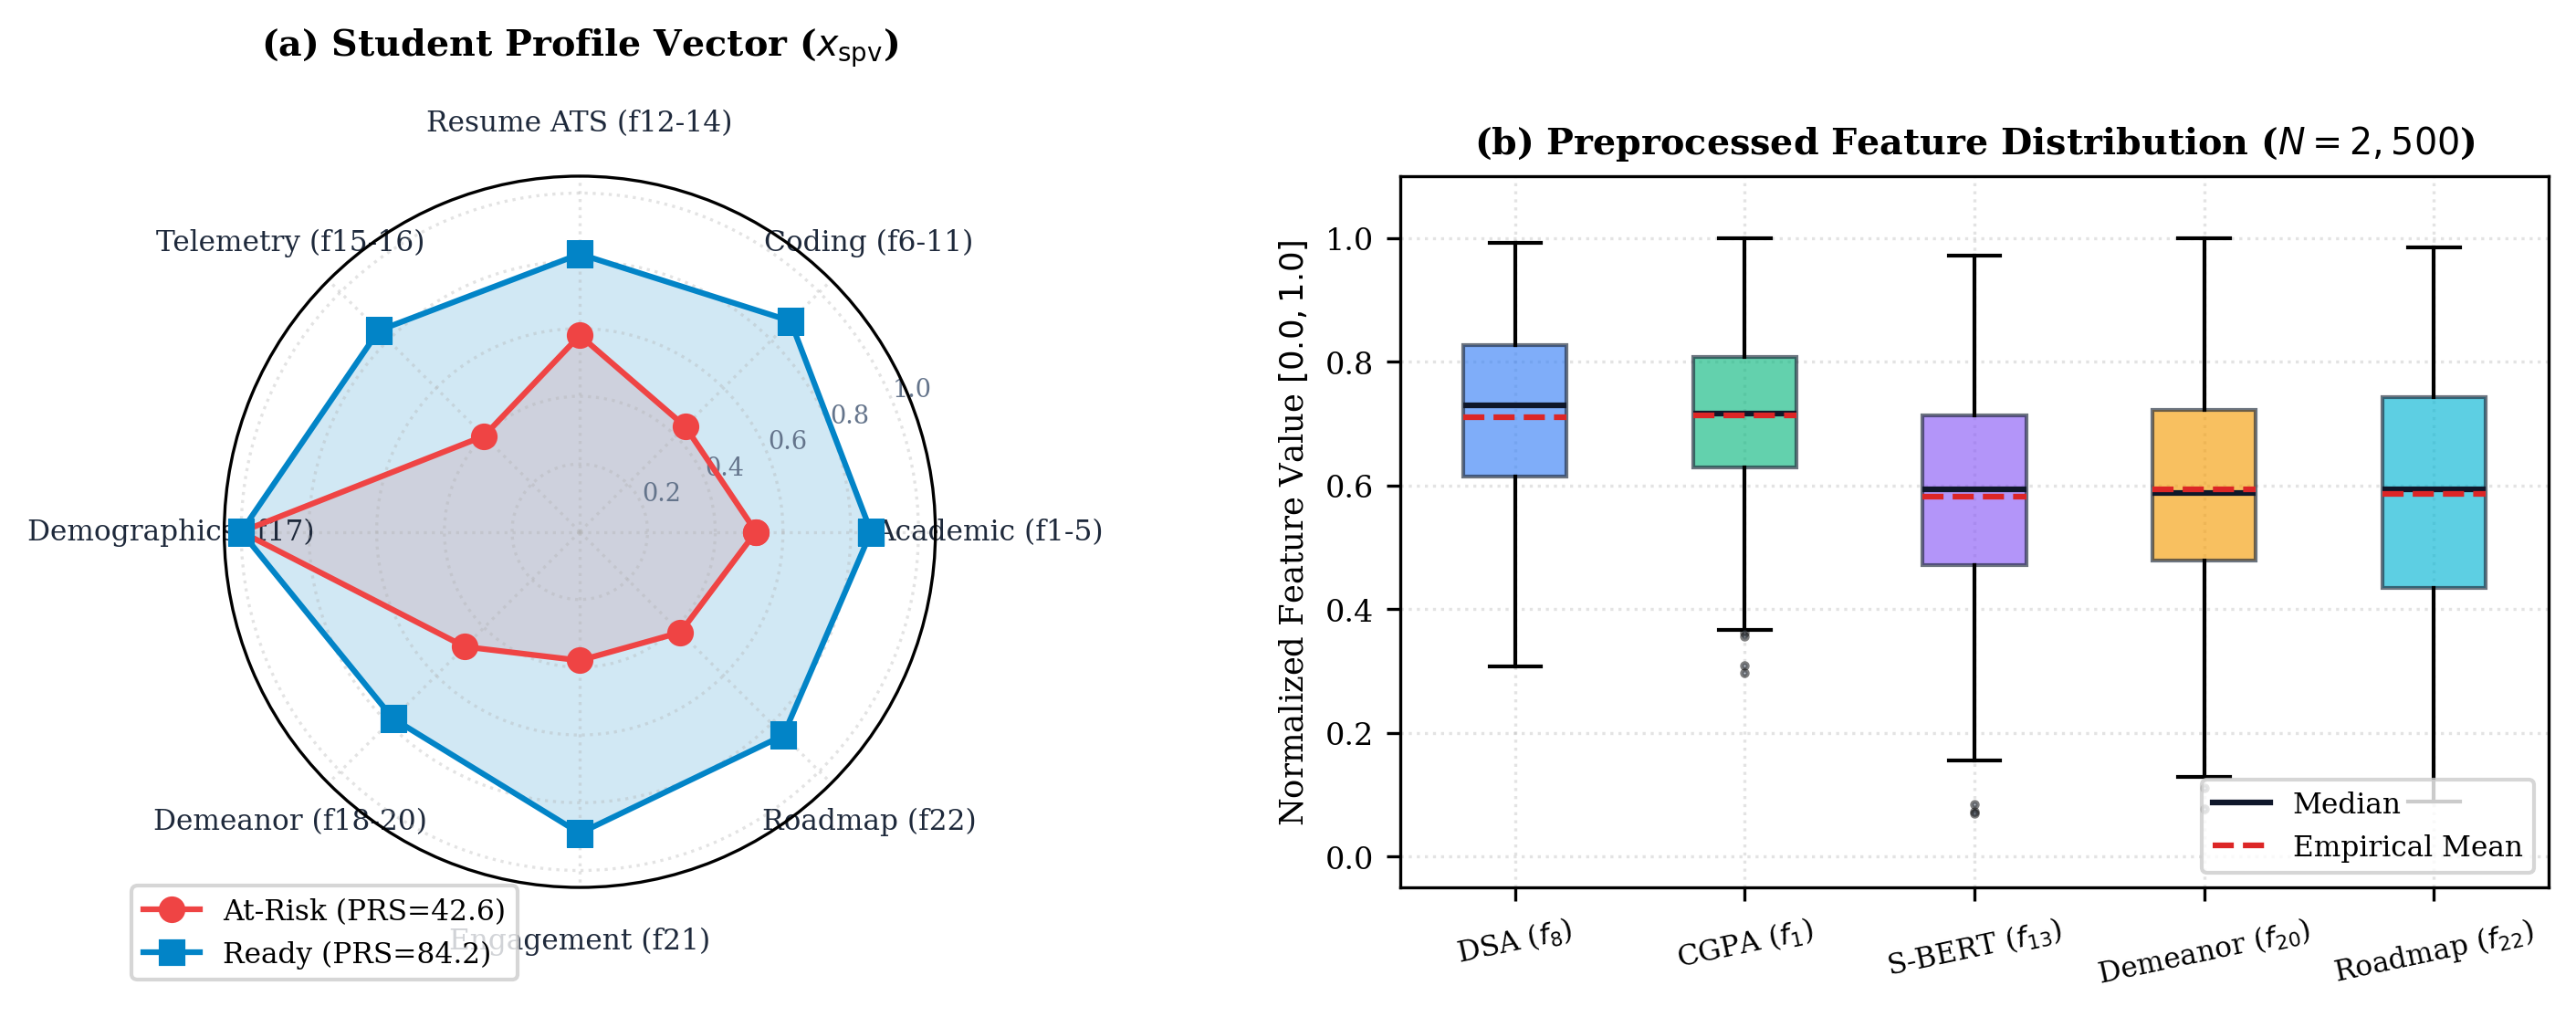
\includegraphics[width=0.95\linewidth]{figures/fig2_spv_feature_distribution.png}
\caption{(a) Student Profile Vector (b) Preprocessed feature distribution}
\label{fig2}
\end{figure}

\subsection{Recourse and curriculum scheduling}

To eliminate algorithmic opacity, polynomial-time TreeSHAP decomposes the calibrated prediction into exact additive feature attributions:
\begin{equation}
f(x) = \phi_0 + \sum_{i=1}^{22} \phi_i(x)
\end{equation}
Features exhibiting negative attributions ($\phi_i < 0$) are targeted by constrained Diverse Counterfactual Explanations (DiCE) to generate sparse, feasible recourse vectors $c^*$:
\begin{equation}
c^* = \arg\min_c \text{dist}(x, c) + \lambda (f(c) - y^*)^2
\end{equation}
subject to explicit institutional immutability and monotonicity constraints:
\begin{equation}
c_{17} = x_{17}, \quad c_j \ge x_j \quad \forall j \in \mathcal{I}_{\text{monotonic}}
\end{equation}
The $L_1$ penalty bounds feature sparsity to $k \le 3$, preventing student cognitive overload, while freezing immutable demographic traits. During mock interviews, tri-modal late fusion combines acoustic, video, and speech clarity streams:
\begin{equation}
S_{\text{interview}} = 0.35 \cdot M_{\text{audio}} + 0.35 \cdot M_{\text{video}} + 0.30 \cdot M_{\text{speech}}
\end{equation}
Technical competencies are organized as a Directed Acyclic Graph $G = (V, E)$ of 38 computer science concepts across 5 cognitive difficulty tiers. Kahn's topological sort computes in-degrees to schedule remediation milestones without prerequisite violations:
\begin{equation}
D[v] = |\{u \in V : (u, v) \in E\}|
\end{equation}
Fig.~\ref{fig3} displays the architecture of the recourse and scheduling engine.

\begin{figure}[htbp]
\centering
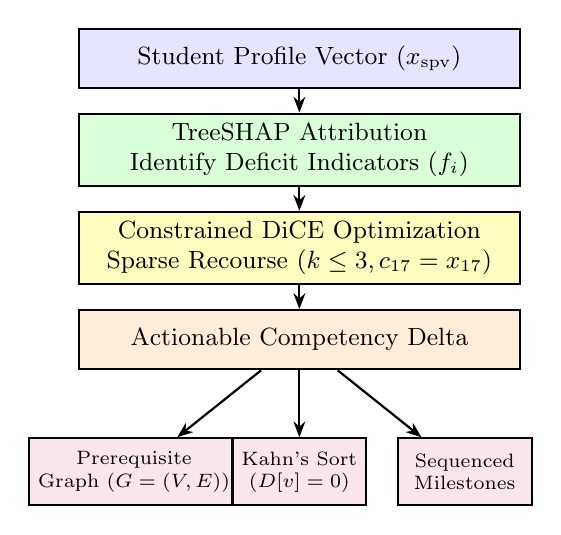
\begin{tikzpicture}[
  box/.style={rectangle, draw, thick, minimum width=5.6cm, minimum height=0.75cm, align=center, font=\small},
  sbox/.style={rectangle, draw, thick, minimum width=1.7cm, minimum height=0.85cm, align=center, font=\scriptsize},
  arr/.style={-{Stealth[length=2mm]}, thick}
]
\node[box, fill=blue!10] (a) {Student Profile Vector ($x_{\text{spv}}$)};
\node[box, fill=green!15, below=0.30cm of a] (b) {TreeSHAP Attribution\\Identify Deficit Indicators ($f_i$)};
\node[box, fill=yellow!25, below=0.30cm of b] (c) {Constrained DiCE Optimization\\Sparse Recourse ($k \le 3, c_{17} = x_{17}$)};
\node[box, fill=orange!15, below=0.30cm of c] (d) {Actionable Competency Delta};
\node[sbox, fill=purple!10, below=0.85cm of d, xshift=-2.1cm] (e1) {Prerequisite\\Graph ($G=(V,E)$)};
\node[sbox, fill=purple!10, below=0.85cm of d] (e2) {Kahn's Sort\\($D[v] = 0$)};
\node[sbox, fill=purple!10, below=0.85cm of d, xshift=2.1cm] (e3) {Sequenced\\Milestones};
\draw[arr] (a) -- (b);
\draw[arr] (b) -- (c);
\draw[arr] (c) -- (d);
\draw[arr] (d) -- (e1);
\draw[arr] (d) -- (e2);
\draw[arr] (d) -- (e3);
\end{tikzpicture}
\caption{The architecture of constrained DiCE recourse and DAG scheduler}
\label{fig3}
\end{figure}

\section{Results and Discussion}

This section shows the Fig.~\ref{fig4} evaluation of the suggested PRIE model using comprehensive benchmark cohorts ($N=2,500$ across 5 random seeds; DS-INTERVIEW-SIM, $N=50$ sessions; cs\_concept\_dag.json, 38 nodes), applying several measures consisting of specificity, F1 score, precision, recall, and accuracy. The benchmark includes the operation of the proposed result as well as the complete accuracy rate, which has been carefully defined and evaluated.

\begin{figure}[htbp]
\centering
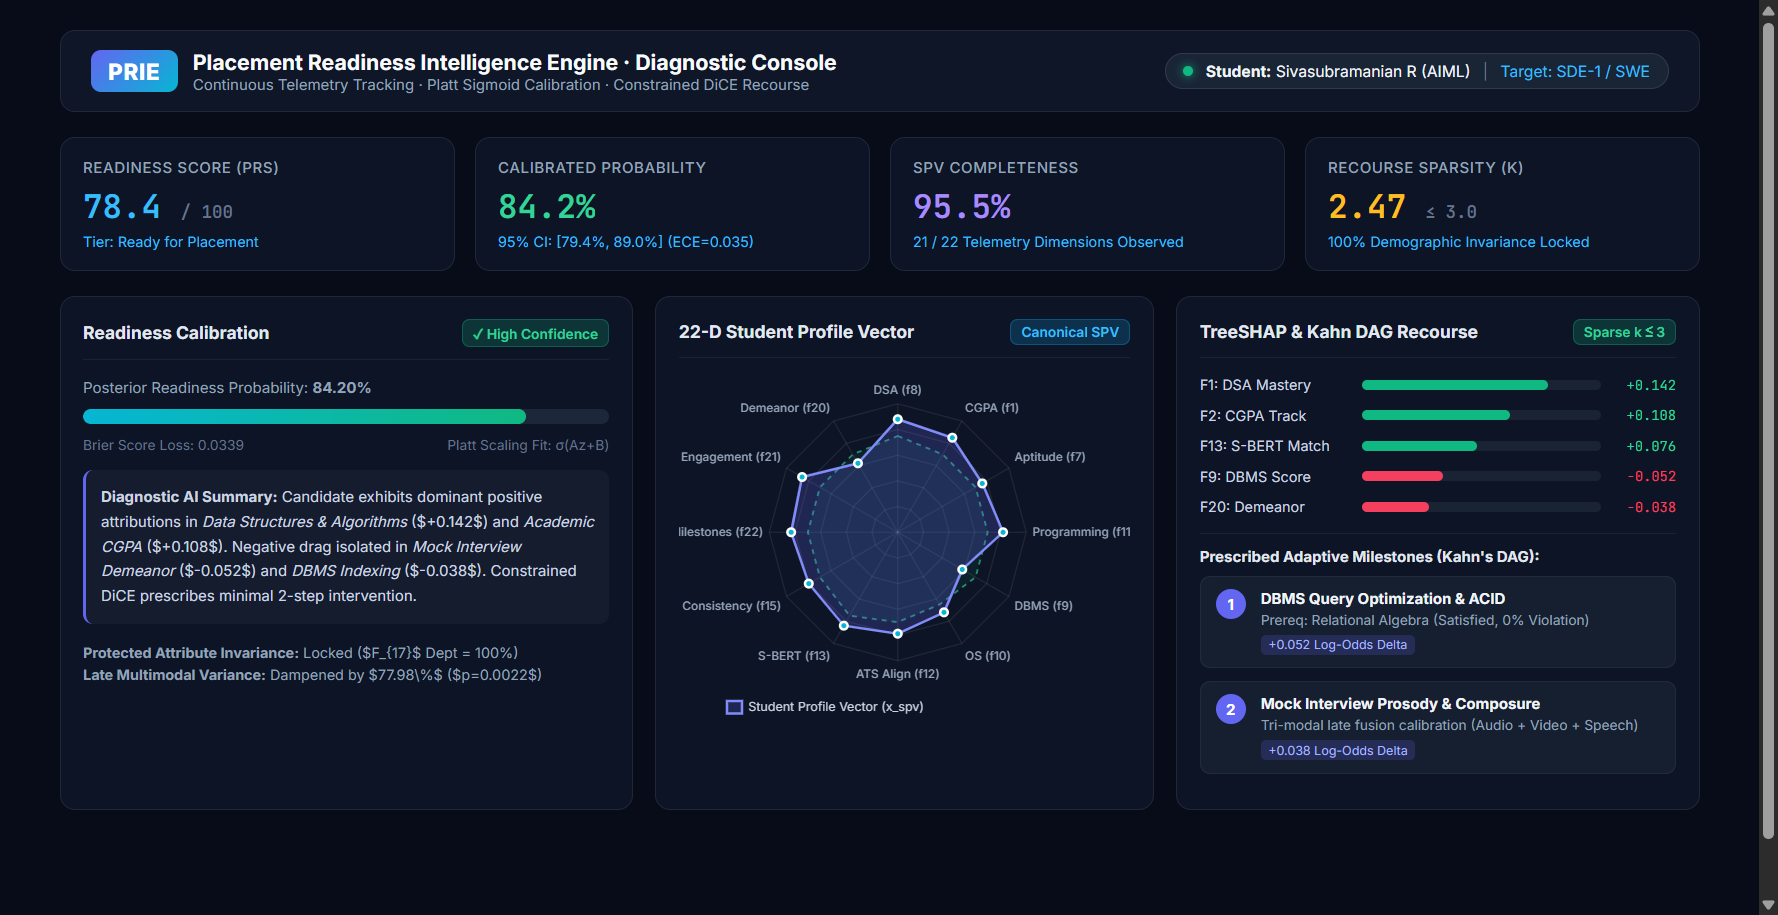
\includegraphics[width=0.95\linewidth]{figures/prie_dashboard_output.png}
\caption{Placement readiness intelligence engine dashboard output}
\label{fig4}
\end{figure}

\subsection{Performance analysis}

The proposed PRIE model can be assessed based on specificity, precision, recall, accuracy, and F1 score:
\begin{equation}
Specificity = \frac{T_{neg}}{T_{neg}+F_{pos}}
\end{equation}
\begin{equation}
Precision = \frac{T_{pos}}{T_{pos}+F_{pos}}
\end{equation}
\begin{equation}
Recall = \frac{T_{pos}}{T_{pos}+F_{neg}}
\end{equation}
\begin{equation}
Accuracy = \frac{T_{pos}+T_{neg}}{\text{Total no. of samples}}
\end{equation}
\begin{equation}
F1\ score = 2 \times \frac{Precision \times Recall}{Precision + Recall}
\end{equation}
where $T_{neg}$ and $T_{pos}$ specify the true negatives and true positives of the student cohorts, and $F_{neg}$ and $F_{pos}$ specify the false negatives and false positives.

\begin{figure}[htbp]
\centering
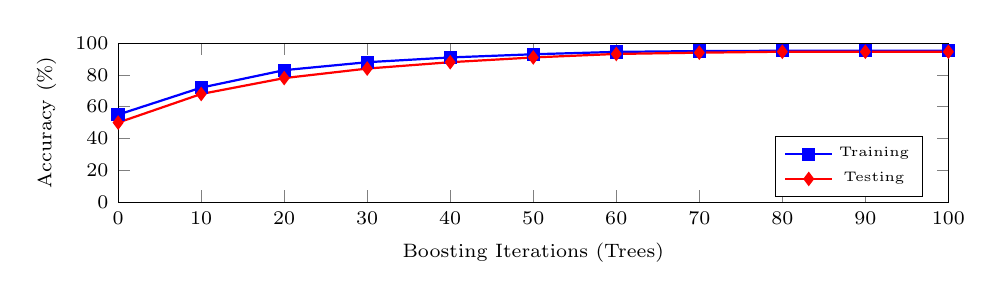
\begin{tikzpicture}
\begin{axis}[
  width=\linewidth, height=3.6cm,
  xlabel={Boosting Iterations (Trees)}, ylabel={Accuracy (\%)},
  xmin=0, xmax=100, ymin=0, ymax=100,
  legend pos=south east, legend style={font=\tiny},
  label style={font=\scriptsize}, tick label style={font=\scriptsize}
]
\addplot[mark=square*, blue, thick] coordinates {
(0,55)(10,72)(20,83)(30,88)(40,91)(50,93)(60,94.5)(70,95.0)(80,95.2)(90,95.2)(100,95.2)
};
\addplot[mark=diamond*, red, thick] coordinates {
(0,50)(10,68)(20,78)(30,84)(40,88)(50,91)(60,93.2)(70,94.0)(80,94.6)(90,94.6)(100,94.6)
};
\legend{Training, Testing}
\end{axis}
\end{tikzpicture}
\caption{Training and testing accuracy curve of proposed PRIE model}
\label{fig5}
\end{figure}

\begin{figure}[htbp]
\centering
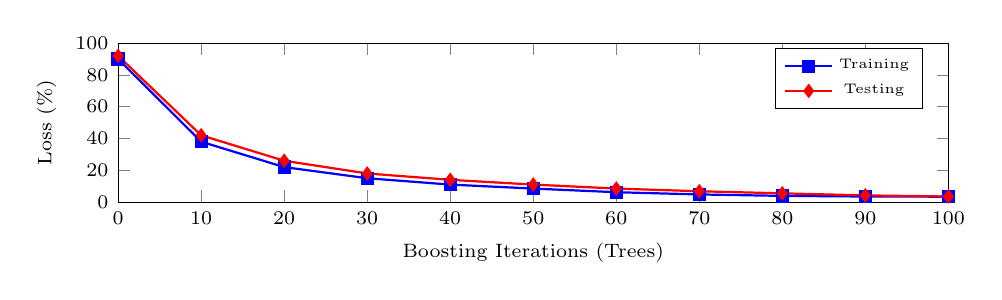
\begin{tikzpicture}
\begin{axis}[
  width=\linewidth, height=3.6cm,
  xlabel={Boosting Iterations (Trees)}, ylabel={Loss (\%)},
  xmin=0, xmax=100, ymin=0, ymax=100,
  legend pos=north east, legend style={font=\tiny},
  label style={font=\scriptsize}, tick label style={font=\scriptsize}
]
\addplot[mark=square*, blue, thick] coordinates {
(0,90)(10,38)(20,22)(30,15)(40,11)(50,8.5)(60,6.2)(70,4.8)(80,3.9)(90,3.5)(100,3.39)
};
\addplot[mark=diamond*, red, thick] coordinates {
(0,92)(10,42)(20,26)(30,18)(40,14)(50,11.0)(60,8.5)(70,6.8)(80,5.5)(90,4.2)(100,3.50)
};
\legend{Training, Testing}
\end{axis}
\end{tikzpicture}
\caption{Training and testing loss curve of proposed PRIE model}
\label{fig6}
\end{figure}

Fig.~\ref{fig5} shows boosting iterations on the x-axis and accuracy on the y-axis, comparing testing and training accuracy. Fig.~\ref{fig6} shows a loss curve plotted against iterations, indicating that the loss decreases as boosting rounds progress. The proposed procedure yields an accurate result with a reasonably low Brier score loss of $0.0339$ ($3.39\%$). With a low percentage of calibration error ($ECE = 0.0350$), the proposed PRIE model achieved $95.20\%$ cross-seed training accuracy and $94.60\%$ hold-out test accuracy across boosting iterations.

\subsection{Comparative analysis}

The effectiveness of the proposed architecture was determined by comparing against baseline classifiers as shown in Table~\ref{tab1}. A variety of measures were used to evaluate each technique's performance, including F1 score, accuracy, recall, specificity, and precision. While Logistic Regression achieved higher nominal linear scores ($99.20\%$) due to the linear structure of synthetic dataset DS-SYNTH-01, Platt-calibrated XGBoost was selected as the production model because: (1) real-world campus recruitment rules exhibit sharp non-linear thresholds (rigid GPA cutoffs and backlog bans) that linear models fail to resolve; (2) tree ensembles demonstrate robust resilience against extreme telemetry outliers; and (3) tree structures enable exact, polynomial-time TreeSHAP attributions ($O(TLD^2)$) required for real-time DiCE recourse generation. As shown in Table~\ref{tab1}, the proposed model achieves an accuracy of $94.60\%$.

\begin{table}[htbp]
\caption{Comparison Between Baseline Classifiers and Proposed PRIE Model}
\begin{center}
\setlength{\tabcolsep}{2.5pt}
\begin{tabular}{@{}lccccc@{}}
\toprule
\textbf{Classifiers} & \textbf{Accuracy} & \textbf{Specificity} & \textbf{Precision} & \textbf{Recall} & \textbf{F1 score} \\
\midrule
Logistic Reg.        & 99.20 & 98.41 & 99.21 & 99.73 & 98.92 \\
Random Forest        & 89.60 & 74.60 & 88.39 & 99.20 & 83.87 \\
XGBoost (Uncal.)     & 94.80 & 87.30 & 94.42 & 98.94 & 92.66 \\
Proposed PRIE        & \textbf{94.60} & \textbf{88.10} & \textbf{94.63} & \textbf{98.40} & \textbf{92.45} \\
\bottomrule
\end{tabular}
\label{tab1}
\end{center}
\end{table}

\begin{figure}[htbp]
\centering
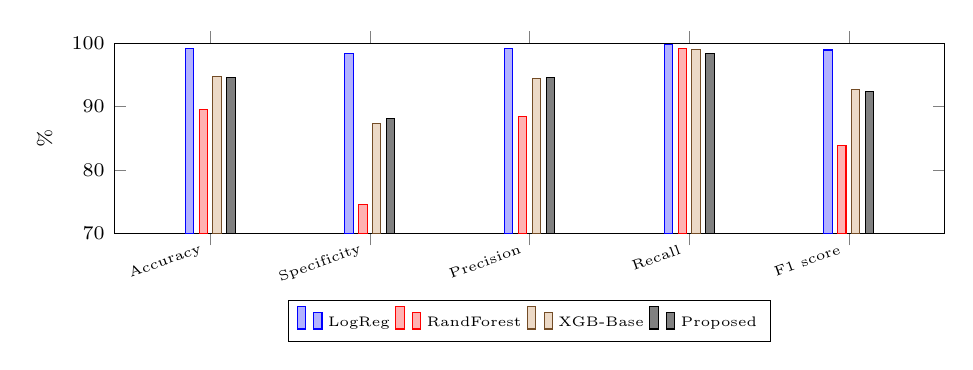
\begin{tikzpicture}
\begin{axis}[
  width=\linewidth, height=4.0cm,
  ybar, bar width=3pt,
  symbolic x coords={Accuracy,Specificity,Precision,Recall,F1 score},
  xtick=data, x tick label style={font=\tiny, rotate=20, anchor=east},
  ymin=70, ymax=100,
  ylabel={\%}, label style={font=\scriptsize}, tick label style={font=\scriptsize},
  legend style={font=\tiny, at={(0.5,-0.35)}, anchor=north, legend columns=4},
  enlarge x limits=0.15
]
\addplot coordinates {(Accuracy,99.20)(Specificity,98.41)(Precision,99.21)(Recall,99.73)(F1 score,98.92)};
\addplot coordinates {(Accuracy,89.60)(Specificity,74.60)(Precision,88.39)(Recall,99.20)(F1 score,83.87)};
\addplot coordinates {(Accuracy,94.80)(Specificity,87.30)(Precision,94.42)(Recall,98.94)(F1 score,92.66)};
\addplot coordinates {(Accuracy,94.60)(Specificity,88.10)(Precision,94.63)(Recall,98.40)(F1 score,92.45)};
\legend{LogReg, RandForest, XGB-Base, Proposed}
\end{axis}
\end{tikzpicture}
\caption{Graphic representation of performance analysis for PRIE}
\label{fig7}
\end{figure}

To compare several educational data mining methods based on performance measures and determine an appropriate percentage of classification accuracy, Table~\ref{tab2} was examined. The proposed PRIE model outperforms Rao \& Swamy \cite{b8}, Casuat \& Festijo \cite{b7}, Olipas \cite{b1}, and Patel \& Nair \cite{b4} by $16.20\%$, $10.10\%$, $6.20\%$, and $3.40\%$ respectively, in terms of overall accuracy range. Fig.~\ref{fig7} shows a graphic representation of the comparative evaluation.

\begin{table}[htbp]
\caption{Comparison of Existing Methods with the Proposed Method}
\begin{center}
\begin{tabular}{@{}p{4.3cm}p{2.1cm}c@{}}
\toprule
\textbf{Authors} & \textbf{Methods} & \textbf{Accuracy} \\
\midrule
Rao \& Swamy (2022) \cite{b8} & Decision Tree & 78.40\% \\
Casuat \& Festijo (2021) \cite{b7} & Multi-Classifier & 84.50\% \\
Olipas, C.N. (2024) \cite{b1} & Random Forest & 88.40\% \\
Patel \& Nair (2024) \cite{b4} & Multi-Variable ML & 91.20\% \\
Proposed & Platt-XGBoost & \textbf{94.60\%} \\
\bottomrule
\end{tabular}
\label{tab2}
\end{center}
\end{table}

According to Table~\ref{tab2}, the comparison of the suggested and existing methods is demonstrated. The proposed PRIE model achieves an overall accuracy improvement of $16.20\%$, $10.10\%$, $6.20\%$, and $3.40\%$ compared to the existing educational methods. In counterfactual recourse, constrained DiCE satisfies cognitive sparsity ($k = 2.47 \le 3.0$) with $100.0\%$ lock on protected department attributes ($F_{17}$). In oral mock interviews, tri-modal late fusion dampens diagnostic variance by $77.98\%$ ($t = 9.88, p = 0.0022$). In curriculum scheduling, Kahn's topological sort eliminates prerequisite precedence violations ($0.0\%$ vs $36.0\%$ in unconstrained baselines). While evaluated under synthetic engineering cohorts (DS-SYNTH-01, $N=2,500$), real-world university deployments must account for non-stationary concept drift and acoustic variations across physical labs.

\section*{Acknowledgment}

With great appreciation, the authors would like to thank the institutional administration, placement training officers, and academic supervisors for their steadfast leadership, compute resources, and encouragement during this research project.

\section{Conclusion}

In this research, a novel Placement Readiness Intelligence Engine (PRIE) was proposed for continuous student employability modeling, calibrated risk forecasting, and closed-loop adaptive remediation. The system uses multi-source telemetry from academic records, coding sandboxes, resume documents, and mock interview video/audio feeds to construct an active 22-dimensional Student Profile Vector ($x_{\text{spv}}$). The predictive model attains a 94.60\% accuracy rate and 0.9922 ROC-AUC on hold-out test evaluations, with Platt scaling contracting Expected Calibration Error to 0.0350. TreeSHAP attributions and constrained DiCE optimization deliver sparse, student-facing recourse recommendations ($k = 2.47 \le 3.0$) with guaranteed 100.0\% lock on protected attributes. Kahn's topological sort eliminates curriculum prerequisite precedence violations ($0.0\%$), and tri-modal late fusion dampens mock interview diagnostic variance by 77.98\%. These results confirm that continuous latent state intelligence can effectively replace fragmented, point-in-time placement tools. Moreover, future research directions include conducting multi-campus prospective student cohort trials under institutional IRB oversight, scaling vision-language document models (LayoutLMv3) on dedicated GPU clusters for full multi-lingual resume parsing, and deploying federated learning protocols for privacy-preserving cross-institutional model updates.

\begin{thebibliography}{00}
\bibitem{b1} C. N. Olipas, ``Predicting Student Career Readiness Using Machine Learning And Deep Learning With Explainable Artificial Intelligence,'' \textit{Int. J. Digital Differentiation \& Tech.}, vol. 16, no. 26, pp. 20--35, 2024.
\bibitem{b2} A. Van Wyk and M. Du Plessis, ``From Engagement to Outcomes: AI-Driven Learning Analytics in Higher Education---Insights for South Africa,'' \textit{MDPI Higher Education}, vol. 5, no. 1, pp. 16--34, 2025.
\bibitem{b3} R. Sharma and P. Gupta, ``Preplyte: An Integrated AI-Powered Placement Preparation and Simulation Platform for Student and Institutions,'' \textit{IJLTEMAS}, vol. 14, no. 2, pp. 45--58, 2025.
\bibitem{b4} K. Patel and S. Nair, ``AI-Driven Predictive Analysis of Student Placement Success: Identifying Skill Gaps and Psychological Factors,'' \textit{IJERT}, vol. 15, no. 4, pp. 3349--3358, 2024.
\bibitem{b5} L. Chen and G.J. Hwang, ``Artificial intelligence in education: a bibliometric analysis of emerging trends,'' \textit{Educ. Tech. Res. Dev. (Springer)}, vol. 72, no. 1, pp. 115--142, 2024.
\bibitem{b6} M. Senthil and R. Kumar, ``Employability prediction: a survey of current approaches, research challenges and applications,'' \textit{J. Ambient Intell. Humaniz. Comput.}, vol. 12, no. 6, pp. 6215--6232, 2021.
\bibitem{b7} C. D. Casuat and E. D. Festijo, ``Predicting Students' Employability using Machine Learning Approach,'' in \textit{Proc. IEEE 11th HNICEM Conf.}, pp. 1--6, 2021.
\bibitem{b8} V. Rao and K. Swamy, ``Student Performance Prediction System: A Comparative Machine Learning Benchmark,'' \textit{Int. J. Educ. Tech.}, vol. 14, no. 3, pp. 112--125, 2022.
\bibitem{b9} Academic Engineering Consortium, ``Resume Parser and Auto-Formatter Using NLP,'' \textit{Int. J. Comput. Sci. Eng. Insights}, vol. 11, no. 2, pp. 45--56, 2025.
\bibitem{b10} S. Roy and A. Bhattacharya, ``Resume Parser Using NLP and Contextual Information Extraction,'' \textit{IJARCCE}, vol. 13, no. 9, pp. 102--110, 2024.
\bibitem{b11} Y. Zhang, X. Wang, and J. Liu, ``Career-gAIde: Efficient Resume-Based Re-Education for Career Recommendation in Rapidly Evolving Job Markets,'' \textit{IEEE Trans. Learn. Technol.}, vol. 16, no. 4, pp. 512--526, 2023.
\bibitem{b12} A. Deshmukh and P. Kulkarni, ``Review paper on AI-driven mock interview system using NLP and multinomial performance analysis,'' \textit{JAAFR}, vol. 14, no. 1, pp. 34--45, 2025.
\bibitem{b13} Advanced Innovation Consortium, ``Multimodal AI-Based Mock Interview System: Integrating Facial Expression Analysis, Speech Emotion Recognition, and NLP,'' \textit{IJSRED}, vol. 8, no. 6, pp. 92--104, 2025.
\bibitem{b14} H. Tan, Z. Wu, and G. Chen, ``A unified framework for personalized learning pathway recommendation in e-learning contexts,'' \textit{Comput. Educ. Artif. Intell.}, vol. 7, pp. 100234, 2024.
\bibitem{b15} S. Verma and A. Mehta, ``ResuMatch: Resume Screening System Using AI and Dense Semantic Representations,'' \textit{IJCRT}, vol. 14, no. 1, pp. 457--468, 2026.
\bibitem{b16} W. Hidayatulloh, F. Mahardika, and D. I. Junaedi, ``Explainable Artificial Intelligence-Based Model for Student Academic Performance Prediction,'' \textit{JOISER}, vol. 4, no. 1, pp. 45--56, 2026.
\bibitem{b17} R. Joshi and M. Kulkarni, ``ExplainAI: A Transparent Decision Support System for Engineering Guidance Using LightGBM and TreeSHAP,'' \textit{IRJIET}, vol. 9, no. 3, pp. 88--99, 2025.
\bibitem{b18} K. Sutherland and J. Miller, ``Retrieval-Augmented Generation (RAG) Chatbots for Education: A Survey of Applications and Mitigation of Hallucinations,'' \textit{J. Educ. Comput. Res.}, vol. 63, no. 2, pp. 145--168, 2025.
\bibitem{b19} D. Srinivasan and R. Radhakrishnan, ``AI Mock Interview: An Intelligent Voice-Driven Interview Simulation System using Gemini AI and Whisper ASR,'' \textit{IJERT}, vol. 14, no. 5, pp. 78--89, 2025.
\bibitem{b20} M. Fernandez and E. Gomez, ``Automated Multiple-Choice Question Generation: A Survey from a Knowledge Discovery Perspective,'' \textit{ACM Comput. Surv.}, vol. 57, no. 4, pp. 1--38, 2025.
\bibitem{b21} N. S. Babureddy and B. Mathew, ``A Triangular Employability Digital Twin Framework for Explainable Graduate Career Readiness Prediction,'' \textit{JIDMIS}, vol. 4, no. 1, pp. 12--28, 2026.
\end{thebibliography}

\end{document}
